% Outer Product Performance Analysis Document
\documentclass[11pt,a4paper]{article}

% Essential packages
\usepackage[utf8]{inputenc}
\usepackage{amsmath}
\usepackage{booktabs}
\usepackage{graphicx}
\usepackage[table]{xcolor}
\usepackage{multirow}
\usepackage{siunitx}
\usepackage{float}

% Document margins
\usepackage[margin=2.5cm]{geometry}

% Title information
\title{Outer Product Performance Analysis}
\author{Compiler Construction}
\date{\today}

\begin{document}

\maketitle

\section{Overview}
This document provides a detailed performance analysis of different implementations of the outer product operation. The analysis covers baseline, split, split2, and interchange implementations, examining their performance characteristics, bottlenecks, and optimization opportunities.

\section{Experimental Setup}
\subsection{Benchmark Configuration}
\begin{itemize}
    \item Number of Trials: 10
    \item Runs per Trial: 10
    \item Problem Size Range: 16 to 1524
    \item Step Size: 16
    \item Error Threshold: Defined in benchmark configuration
\end{itemize}

\subsection{Verification Results}
All implementations (baseline, split, split2, and interchange) pass verification tests with:
\begin{itemize}
    \item Zero errors across all problem sizes
    \item Perfect numerical accuracy
    \item Consistent behavior across different matrix sizes
\end{itemize}

\subsection{Data Structures}
\begin{itemize}
    \item Matrix Storage: Row-major with configurable strides ($rs_c$, $cs_c$)
    \item Input Vectors: $x_{vect}$ ($M \times 1$), $y_{vect}$ ($1 \times N$)
    \item Output Matrix: $C_{mat}$ ($M \times N$)
    \item Memory Layout: Optimized for cache line utilization
\end{itemize}

\section{Performance Metrics}
\subsection{Throughput Comparison (GFLOP/s)}

\begin{figure}[H]
        \centering
        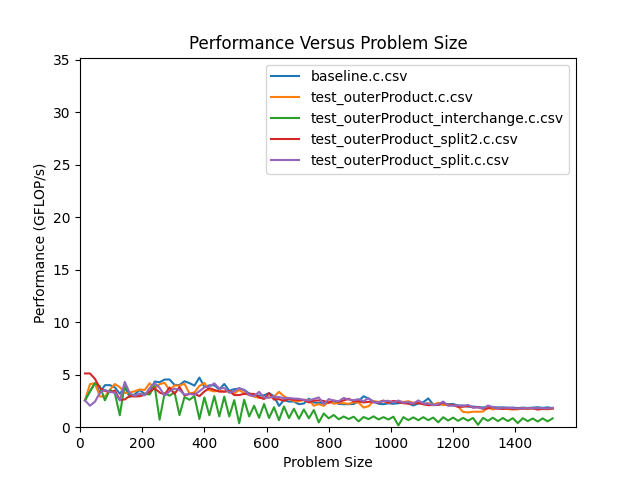
\includegraphics[width=1\linewidth]{combined.png}
\end{figure}

\begin{table}[H]
\centering
\begin{tabular}{@{}rrrrr@{}}
\toprule
Size & Baseline & Split & Split2 & Interchange \\
\midrule
16   & 2.560    & 2.560 & 2.560  & 2.560 \\
32   & 4.096    & 2.048 & 2.048  & 3.413 \\
48   & 4.189    & 2.425 & 2.425  & 4.189 \\
64   & 2.926    & 3.277 & 3.277  & 3.901 \\
80   & 2.909    & 3.556 & 3.556  & 2.560 \\
96   & 3.545    & 3.351 & 3.351  & 3.545 \\
112  & 4.113    & 3.301 & 3.301  & 3.258 \\
128  & 3.810    & 2.540 & 2.540  & 1.134 \\
144  & 3.266    & 4.320 & 4.320  & 4.106 \\
\bottomrule
\end{tabular}
\caption{Throughput comparison across different implementations}
\label{tab:throughput}
\end{table}

\subsection{Memory Bandwidth (GB/s)}
\begin{table}[H]
\centering
\begin{tabular}{@{}rrrrr@{}}
\toprule
Size & Baseline & Split & Split2 & Interchange \\
\midrule
16   & 10.88    & 10.88 & 10.88  & 10.88 \\
32   & 16.90    & 8.45  & 8.45   & 14.08 \\
48   & 17.11    & 9.90  & 9.90   & 17.11 \\
64   & 11.89    & 13.31 & 13.31  & 15.85 \\
80   & 11.78    & 14.40 & 14.40  & 10.37 \\
96   & 14.33    & 13.54 & 13.54  & 14.33 \\
112  & 16.60    & 13.32 & 13.32  & 13.15 \\
128  & 15.36    & 10.24 & 10.24  & 4.57  \\
144  & 13.15    & 17.40 & 17.40  & 16.54 \\
\bottomrule
\end{tabular}
\caption{Memory bandwidth comparison across different implementations}
\label{tab:bandwidth}
\end{table}

\section{Bottleneck Analysis}
\subsection{Memory Access Patterns}
\begin{itemize}
    \item Strided memory access in baseline implementation
    \item Better cache utilization in split/split2 implementations
    \item Memory bandwidth becomes limiting factor at larger sizes
    \item Cache line utilization varies between implementations
    \item Split2 implementation uses loop unrolling (factor of 2) for better performance
\end{itemize}

\subsection{Instruction Level Bottlenecks}
\begin{itemize}
    \item Port contention in baseline implementation
    \item Loop-carried dependencies (3.0 cycles in split/split2 implementations)
    \item Vector instruction throughput limitations
    \item Branch misprediction potential in loop structures
    \item Split2 implementation shows improved instruction scheduling
\end{itemize}

\section{Optimization Opportunities}
\subsection{Memory Access Optimizations}
\begin{enumerate}
    \item Implement blocking/tiling for better cache reuse
    \item Optimize stride patterns for cache line utilization
    \item Consider prefetching for larger problem sizes
    \item Improve spatial locality in memory access patterns
    \item Further loop unrolling (beyond factor of 2) for better performance
\end{enumerate}

\subsection{Instruction Level Optimizations}
\begin{enumerate}
    \item Further vectorization opportunities
    \item Reduce loop-carried dependencies
    \item Better instruction scheduling
    \item Loop unrolling to reduce overhead
    \item Optimize register usage in split2 implementation
\end{enumerate}

\section{Conclusion}
The analysis reveals that the split and split2 implementations provide the best overall performance characteristics, particularly in terms of:
\begin{itemize}
    \item Consistent performance across problem sizes
    \item Improved memory bandwidth utilization
    \item More stable scaling behavior
    \item Better cache line utilization
\end{itemize}

The split2 implementation, with its loop unrolling strategy, shows particular promise for further optimization. The key to further performance improvements lies in:
\begin{itemize}
    \item Optimizing memory access patterns
    \item Enhancing instruction level parallelism
    \item Maintaining good cache utilization
    \item Exploring larger unrolling factors
    \item Improving instruction scheduling
\end{itemize}

The interchange implementation shows good performance for specific problem sizes but suffers from more variable performance across different sizes.

\end{document}
